\documentclass[11pt]{article}
\usepackage[utf8]{inputenc}
\usepackage[T1]{fontenc}
\usepackage[spanish,es-nodecimaldot]{babel}
\usepackage[margin=1.85cm,headheight=15pt]{geometry}
\usepackage{lmodern}
\usepackage{microtype}
\usepackage{graphicx}
\usepackage{array}
\usepackage{booktabs}
\usepackage{longtable}
\usepackage{tabularx}
\usepackage{enumitem}
\usepackage{float}
\usepackage{caption}
\usepackage{xcolor}
\usepackage{xurl}
\usepackage{fancyhdr}
\usepackage{titlesec}
\usepackage{amsmath}
\usepackage{amssymb}
\usepackage{hyperref}

\graphicspath{{../screenshots/}{../doc_figures/}{../sprott/images/generated/}}

\definecolor{AzulProfundo}{HTML}{17365D}
\definecolor{AzulMedio}{HTML}{2C6E9B}
\definecolor{Turquesa}{HTML}{198F8A}
\definecolor{Naranja}{HTML}{E28A36}
\definecolor{FondoAzul}{HTML}{EDF5FA}
\definecolor{FondoVerde}{HTML}{EEF8F5}
\definecolor{FondoNaranja}{HTML}{FFF5E9}
\definecolor{GrisTexto}{HTML}{27313B}
\definecolor{GrisClaro}{HTML}{F5F7F9}

\hypersetup{
  colorlinks=true,
  linkcolor=AzulProfundo,
  urlcolor=AzulMedio,
  citecolor=Turquesa,
  pdftitle={Manual de usuario de Toolbox Chaos},
  pdfauthor={Maria Fernanda Moreno Lopez},
  pdfsubject={Guia pedagogica para operar Toolbox Chaos}
}

\setlength{\parindent}{0pt}
\setlength{\parskip}{0.48em}
\setlength{\emergencystretch}{2em}
\setlist[itemize]{leftmargin=1.5em,itemsep=0.18em,topsep=0.25em}
\setlist[enumerate]{leftmargin=1.7em,itemsep=0.25em,topsep=0.25em}
\renewcommand{\arraystretch}{1.18}

\titleformat{\section}
  {\Large\bfseries\color{AzulProfundo}}{\thesection}{0.65em}{}
\titleformat{\subsection}
  {\large\bfseries\color{AzulMedio}}{\thesubsection}{0.55em}{}
\titleformat{\subsubsection}
  {\normalsize\bfseries\color{Turquesa}}{}{0pt}{}
\titleformat{\paragraph}[block]
  {\normalsize\bfseries\color{Turquesa}}{}{0pt}{}
\titlespacing*{\paragraph}{0pt}{0.8em}{0.25em}

\pagestyle{fancy}
\fancyhf{}
\fancyhead[L]{\small Toolbox Chaos}
\fancyhead[R]{\small Manual de usuario}
\fancyfoot[L]{\small Fyskode}
\fancyfoot[C]{\thepage}
\fancyfoot[R]{\small v0.2.0}
\fancypagestyle{plain}{
  \fancyhf{}
  \fancyhead[L]{\small Toolbox Chaos}
  \fancyhead[R]{\small Manual de usuario}
  \fancyfoot[L]{\small Fyskode}
  \fancyfoot[C]{\thepage}
  \fancyfoot[R]{\small v0.2.0}
}

\newcommand{\boton}[1]{\textsf{\itshape #1}}
\newcommand{\campo}[1]{\textsf{#1}}
\newcommand{\archivo}[1]{\nolinkurl{#1}}
\newcommand{\urlimpresa}[1]{\href{#1}{\nolinkurl{#1}}}
\newcommand{\paso}[1]{\textcolor{AzulProfundo}{\bfseries #1}}
\newcommand{\manualteorico}{\href{run:manual_teorico_pedagogico.pdf}{\emph{Manual teórico pedagógico}} (\nolinkurl{manual_teorico_pedagogico.pdf})}
\newcommand{\manualsprott}{\href{run:manual_explorador_sprott.pdf}{\emph{Manual pedagógico del Explorador Sprott}} (\nolinkurl{manual_explorador_sprott.pdf})}

\newenvironment{cajaazul}[1]
{\begin{center}\begin{minipage}{0.93\linewidth}\color{GrisTexto}
\textcolor{AzulMedio}{\rule{\linewidth}{0.8pt}}\par\smallskip
\textcolor{AzulProfundo}{\bfseries #1}\par\smallskip}
{\par\smallskip\textcolor{AzulMedio}{\rule{\linewidth}{0.8pt}}\end{minipage}\end{center}}

\newenvironment{cajaverde}[1]
{\begin{center}\begin{minipage}{0.93\linewidth}\color{GrisTexto}
\textcolor{Turquesa}{\rule{\linewidth}{0.8pt}}\par\smallskip
\textcolor{Turquesa}{\bfseries #1}\par\smallskip}
{\par\smallskip\textcolor{Turquesa}{\rule{\linewidth}{0.8pt}}\end{minipage}\end{center}}

\newenvironment{cajaalerta}[1]
{\begin{center}\begin{minipage}{0.93\linewidth}\color{GrisTexto}
\textcolor{Naranja}{\rule{\linewidth}{0.8pt}}\par\smallskip
\textcolor{Naranja}{\bfseries #1}\par\smallskip}
{\par\smallskip\textcolor{Naranja}{\rule{\linewidth}{0.8pt}}\end{minipage}\end{center}}

\newcommand{\capturacompleta}[2]{
\begin{figure}[H]
  \centering
  \includegraphics[width=0.98\linewidth]{#1}
  \caption{#2}
\end{figure}}

\newcommand{\figuradidactica}[2]{
\begin{figure}[H]
  \centering
  \includegraphics[width=0.94\linewidth,height=0.42\textheight,keepaspectratio]{#1}
  \caption{#2}
\end{figure}}

\begin{document}
\hypersetup{pageanchor=false}

\begin{titlepage}
\thispagestyle{empty}
\color{GrisTexto}
\vspace*{0.35cm}
{\Huge\bfseries\color{AzulProfundo} Manual de usuario de Toolbox Chaos\par}
\vspace{0.35cm}
 {\Large Instalación, simulación, análisis y exportación reproducible de sistemas dinámicos\par}
\vspace{0.55cm}
{\large Fyskode Chaotic Systems Toolbox 0.2.0\par}
\vspace{0.8cm}
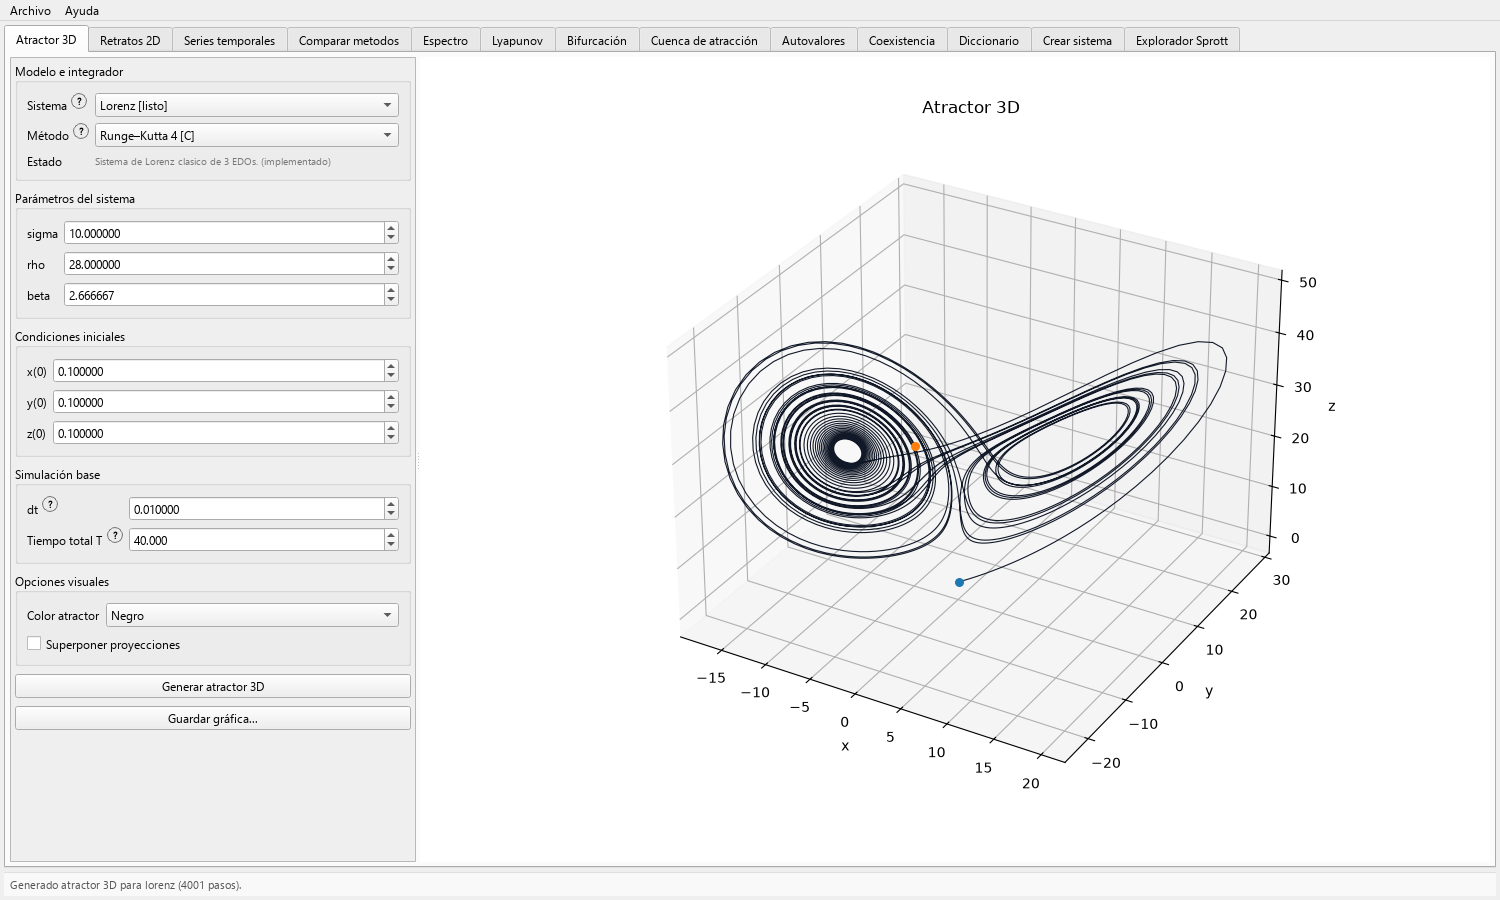
\includegraphics[width=\linewidth]{gui_attractor_3d.png}
\vfill
\begin{cajaazul}{Instalación y uso de Toolbox Chaos}
Este documento enseña a operar la interfaz gráfica desde la instalación hasta la exportación de resultados. Las explicaciones matemáticas extensas se encuentran en el \manualteorico; el tratamiento especializado de códigos compactos se encuentra en el \manualsprott.
\end{cajaazul}
\vfill
{\large Maria Fernanda Moreno Lopez (Fer Moreno)\par}
{\small \urlimpresa{https://search.fyskode.com/toolbox_chaos}\par}
{\small Agosto de 2026\par}
\end{titlepage}

\hypersetup{pageanchor=true}
\pagenumbering{roman}
\tableofcontents
\clearpage
\pagenumbering{arabic}

\section{Instalación y controles de Toolbox Chaos}

Toolbox Chaos organiza el trabajo en trece pestañas. El proyecto se presenta públicamente con ese nombre, mientras que la barra de título y el acceso directo muestran \emph{Chaos Toolbox}; ambas denominaciones identifican la misma aplicación gráfica. Varias pestañas comparten el selector de sistema, parámetros, condiciones iniciales y paso temporal; otras reúnen laboratorios especializados. El uso se explica a partir de una trayectoria de Lorenz que se conserva para generar distintas representaciones. A partir de ese cálculo se introducen los barridos de parámetros, las cuencas de atracción, los exponentes de Lyapunov, la coexistencia y la definición de modelos propios.

Los nombres de controles aparecen en letra sans serif cursiva, por ejemplo \boton{Generar atractor 3D}. Cuando el texto indica \emph{pulse}, se refiere a activar ese control en la interfaz. Los nombres de archivos y comandos aparecen en letra monoespaciada.

\begin{cajaverde}{Operaciones descritas en el manual}
La persona usuaria podrá reproducir una simulación, conservar sus parámetros, generar figuras comparables, distinguir entre una visualización y una conclusión científica, y preparar un paquete mínimo de datos para compartir su experimento.
\end{cajaverde}

Antes de instalar conviene distinguir los tres documentos que acompañan el software. Esta separación evita interrumpir un procedimiento de uso con una demostración extensa y, al mismo tiempo, permite continuar el estudio cuando una gráfica necesita fundamento adicional.

\begin{tabularx}{\linewidth}{>{\raggedright\arraybackslash}p{0.25\linewidth}X}
\toprule
Documento & Contenido principal \\
\midrule
\emph{Manual de usuario} (este archivo) & ¿Qué control debo usar y en qué orden para obtener, guardar y repetir un resultado? \\
\manualteorico & ¿Qué significan matemáticamente las trayectorias, atractores, espectros, bifurcaciones, cuencas, autovalores y exponentes de Lyapunov? \\
\manualsprott & ¿Cómo se decodifican, simulan, interpretan y documentan los códigos compactos inspirados en Sprott? \\
\bottomrule
\end{tabularx}

\paragraph{Instalación en Windows.}

El instalador de Windows integra la aplicación, el entorno de Python y las bibliotecas necesarias para ejecutar la distribución empaquetada. Por ello, la instalación habitual se completa con el ejecutable distribuido.

\begin{enumerate}
  \item Abra la página de versiones: \urlimpresa{https://github.com/Xerkkun/Toolbox-chaos/releases}.
  \item Descargue \archivo{chaos-toolbox-v0.2.0-windows-x64-setup.exe}.
  \item Compruebe que el archivo provenga de la página anterior. Si la publicación incluye una suma SHA-256, compárela antes de ejecutar el instalador.
  \item Ejecute el archivo, acepte la ubicación propuesta o elija otra carpeta y complete el asistente.
  \item Abra \emph{Chaos Toolbox} desde el menú Inicio o el acceso directo creado por el instalador.
\end{enumerate}

\begin{cajaalerta}{Advertencias de reputación en Windows}
Windows puede mostrar una advertencia de reputación cuando un ejecutable carece de una firma reconocida por el equipo. Compruebe el origen: continúe con el instalador obtenido desde la URL oficial indicada arriba y, cuando esté disponible, verifique su suma de comprobación.
\end{cajaalerta}

\paragraph{Instalación con Python.}

Esta ruta es útil para docencia, desarrollo o entornos donde se administran paquetes de Python. Requiere Python 3.11 o posterior.

Desde PyPI:
\begin{verbatim}
python -m pip install --upgrade pip
python -m pip install chaos-toolbox
chaos-toolbox
\end{verbatim}

Página explícita del paquete: \urlimpresa{https://pypi.org/project/chaos-toolbox/}.

Desde el repositorio:
\begin{verbatim}
git clone https://github.com/Xerkkun/Toolbox-chaos.git
cd Toolbox-chaos
python -m venv .venv
.venv\Scripts\Activate.ps1
python -m pip install --upgrade pip
python -m pip install .
chaos-toolbox
\end{verbatim}

La instalación normal declara e instala la versión compatible de \archivo{hidden-attractors-fo}; este paquete funciona como motor matemático. La persona usuaria opera Toolbox Chaos mediante su interfaz para seguir los laboratorios de este manual.

\paragraph{Inicio de la aplicación.}

La ventana muestra la barra de menús \campo{Archivo} y \campo{Ayuda}, trece pestañas y una barra de estado inferior. En \campo{Atractor 3D}, el selector inicial incluye \campo{Lorenz [listo]}. Cuando el área gráfica esté vacía, pulse \boton{Generar atractor 3D} para iniciar el primer cálculo.

\paragraph{Pestañas y funciones de la interfaz.}

\begin{longtable}{>{\raggedright\arraybackslash}p{0.20\linewidth}>{\raggedright\arraybackslash}p{0.27\linewidth}>{\raggedright\arraybackslash}p{0.43\linewidth}}
\toprule
Pestaña & Producto principal & Cuándo usarla \\
\midrule
\endhead
\campo{Atractor 3D} & Trayectoria tridimensional & Primer reconocimiento geométrico de un flujo o de una trayectoria con tres componentes. \\
\campo{Retratos 2D} & Proyecciones por pares & Comparar planos de fase y revelar estructura que puede ocultarse en una vista 3D. \\
\campo{Series temporales} & Estado contra tiempo o iteración & Examinar transitorios, amplitud, alternancia, saturación y escalas temporales. \\
\campo{Comparar metodos} & Tres series por integrador & Comprobar sensibilidad numérica entre Euler, Heun y RK4 con el mismo contrato. \\
\campo{Espectro} & PSD de Welch o espectro de amplitud & Localizar componentes dominantes y comparar contenido frecuencial después de retirar un transitorio. \\
\campo{Lyapunov} & Espectro finito y curvas de convergencia & Estimar separación de perturbaciones en flujos ODE enteros de tres dimensiones registrados. \\
\campo{Bifurcación} & Barrido de un parámetro & Reconocer cambios cualitativos, ventanas y coexistencia al variar un parámetro. \\
\campo{Cuenca de atracción} & Clasificación de una malla de condiciones iniciales & Estudiar sensibilidad al estado inicial y fronteras entre destinos calculados. \\
\campo{Autovalores} & Equilibrios y plano complejo & Revisar estabilidad local de equilibrios de flujos ODE compatibles. \\
\campo{Coexistencia} & Atractores reportados para un mismo conjunto de parámetros & Reproducir casos catalogados y enviarlos a otras pestañas. \\
\campo{Manuales} & Usuario, teoría y Explorador Sprott & Consultar dentro de la aplicación los tres documentos pedagógicos que acompañan el trabajo. \\
\campo{Crear sistema} & Trayectoria de un flujo o mapa definido sin código Python & Probar ecuaciones propias mediante el analizador restringido y guardar la definición en JSON. \\
\campo{Explorador Sprott} & Decodificación, simulación, estilo y galería de códigos compactos & Recuperar con fines didácticos el método de exploración de Sprott y extenderlo con herramientas actuales. \\
\bottomrule
\end{longtable}

\capturacompleta{gui_full_window_current.png}{Ventana completa de Toolbox Chaos. Las pestañas forman una ruta de trabajo común y el panel izquierdo conserva el sistema, los parámetros y el contrato numérico de la vista activa.}

\begin{cajaazul}{Datos locales y trayectoria compartida}
Las pestañas con el panel \campo{Modelo e integrador} mantienen sus propios valores. Seleccionar un sistema carga los valores predeterminados de esa pestaña. En cambio, los botones \boton{Usar última trayectoria} recuperan explícitamente la trayectoria compartida más reciente para visualizar el cálculo ya realizado.
\end{cajaazul}

\section{Trayectoria de Lorenz y reutilización de datos}

El primer ejercicio genera una trayectoria reproducible con los valores predeterminados y permite reconocer la relación entre el modelo, el integrador, las condiciones iniciales y la malla temporal.

\begin{enumerate}
  \item Abra \campo{Atractor 3D}.
  \item En \campo{Sistema}, elija \campo{Lorenz [listo]}.
  \item En \campo{Método}, elija \campo{Runge--Kutta 4 [C]}.
  \item Confirme los parámetros \(\sigma=10\), \(\rho=28\) y \(\beta=2.666667\).
  \item Confirme \(x(0)=y(0)=z(0)=0.1\), \campo{dt} = 0.01 y \campo{Tiempo total T} = 40.
  \item Elija un \campo{Color atractor}. Active \campo{Superponer proyecciones} si desea ver sombras geométricas sobre los planos coordenados.
  \item Pulse \boton{Generar atractor 3D}.
\end{enumerate}

La barra inferior debe informar que se generó el atractor y el área derecha debe mostrar los dos lóbulos característicos. El punto inicial y el final ayudan a seguir el sentido de la trayectoria.

\capturacompleta{gui_attractor_3d.png}{Pestaña \campo{Atractor 3D} después de calcular el sistema de Lorenz con RK4. El panel izquierdo conserva el contrato numérico necesario para repetir la figura.}

\begin{cajaalerta}{Límites de la visualización del atractor}
La identificación de caos y atracción requiere comparar integradores, retirar el transitorio y revisar la convergencia de los exponentes de Lyapunov. La forma de la curva orienta esa revisión inicial.
\end{cajaalerta}

\paragraph{Retratos 2D, series temporales y espectro.}

La simulación de Lorenz calculada en la sección anterior queda disponible como última trayectoria. Reutilizarla permite comparar visualizaciones sin introducir diferencias por una nueva ejecución.

En \campo{Retratos 2D}, pulse \boton{Usar última trayectoria}. En \campo{Proyecciones 2D} puede conservar únicamente las parejas que necesite; para tres variables se ofrecen \(x\)-\(y\), \(x\)-\(z\) y \(y\)-\(z\). El selector \campo{Color} modifica la presentación y conserva los datos calculados. Cuando la composición sea adecuada, \boton{Guardar gráfica...} exporta el panel. \boton{Generar retratos 2D} calcula una trayectoria nueva con los valores locales de la pestaña, mientras que \boton{Usar última trayectoria} dibuja los datos ya compartidos.

\capturacompleta{gui_phase_portraits_2d.png}{Retratos de fase del mismo experimento de Lorenz en tres planos. Las proyecciones muestran el mismo conjunto de estados desde pares de coordenadas distintos.}

Continúe en \campo{Series temporales} y pulse \boton{Usar última trayectoria}. Las vistas separadas de \(x(t)\), \(y(t)\) y \(z(t)\) permiten reconocer el tramo inicial de adaptación y compararlo con el resto de la simulación. Los selectores de color ayudan a distinguir variables sin alterar la trayectoria; \boton{Guardar gráfica...} conserva la composición mostrada.

\capturacompleta{gui_time_series.png}{Series temporales de Lorenz. La vista extendida en el eje horizontal permite reconocer el transitorio inicial y la evolución irregular posterior.}

La misma trayectoria puede examinarse por variable de estado en \campo{Espectro}. Después de pulsar \boton{Usar última trayectoria}, seleccione en \campo{Método} la opción \campo{PSD de Welch (recomendado)} y ajuste \campo{Descartar transitorio (s)} para excluir el arranque. Durante la primera lectura es razonable dejar \campo{Frecuencia mínima (0=auto)} y \campo{Frecuencia máxima (0=auto)} en cero. \boton{Calcular FFT/PSD} vuelve a calcular desde el panel de la pestaña y \boton{Guardar gráfica...} exporta la salida. Para analizar amplitudes de la transformada rápida de Fourier, repita la observación con \campo{Espectro de amplitud}.

\capturacompleta{gui_welch_psd.png}{PSD de Welch para cada variable del sistema de Lorenz. La pestaña también ofrece el espectro de amplitud de una FFT unilateral.}

\begin{cajaverde}{Estabilidad del contenido espectral}
¿Los máximos espectrales se conservan al aumentar el tiempo total? Describa como dependiente del contrato numérico toda característica que cambie con la longitud de la señal o el transitorio descartado, y reserve la confirmación para las que persisten bajo esas variaciones.
\end{cajaverde}

\paragraph{Comparación de integradores.}

En sistemas caóticos, dos trayectorias numéricas pueden separarse aunque los métodos sean correctos. La comparación estudia el efecto de la discretización mediante la escala global, la estructura de fase y los diagnósticos declarados. Abra \campo{Comparar metodos}, seleccione \campo{Lorenz [listo]} y reproduzca los parámetros, condiciones iniciales, \campo{dt} y \campo{Tiempo total T} del laboratorio. En \campo{Integradores a comparar}, active \campo{Euler explícito}, \campo{Heun / Euler mejorado (RK2)} y \campo{Runge--Kutta 4}, asigne colores distintos y pulse \boton{Comparar integradores}. Una segunda ejecución con \campo{dt} menor permite comparar cuánto tiempo permanecen próximas las curvas y si se conserva la escala global de cada variable.

\capturacompleta{gui_method_comparison.png}{Comparación de Euler, Heun y RK4 para las tres variables de Lorenz. La separación tardía debe interpretarse junto con el paso, el horizonte y la sensibilidad dinámica.}

\begin{cajaazul}{Datos necesarios para reproducir la simulación}
Anote siempre sistema, parámetros, estado inicial, método, \(dt\), tiempo total, versión del programa y fecha de ejecución. Ese contrato permite repetir el cálculo y revisar la figura en su contexto numérico.
\end{cajaazul}

\section{Bifurcaciones, cuencas, Lyapunov y equilibrios}

Una trayectoria permite reconocer la evolución de un estado inicial, pero muchas preguntas de investigación requieren relacionar varias trayectorias, parámetros o escalas locales. Las siguientes herramientas se presentan en un orden deliberado: primero se estudia el cambio producido por un parámetro, después la dependencia respecto al estado inicial y, finalmente, se combinan diagnósticos globales y locales.

\paragraph{Diagrama de bifurcación.}

La pestaña \campo{Bifurcación} barre un parámetro del sistema, descarta un transitorio y conserva eventos o últimos valores de la variable observada. Es una herramienta para localizar regiones que merecen simulaciones más detalladas.

Para el ejercicio, seleccione \campo{Logistico [listo]}, elija \campo{r} como \campo{Parámetro de bifurcación} y \campo{x} como \campo{Variable observada}. \campo{Mínimo}, \campo{Máximo} y \campo{N (Parámetros)} determinan el intervalo y su muestreo; conviene empezar con pocos parámetros y aumentar la resolución solo después de confirmar que el intervalo es informativo. Antes de pulsar \boton{Calcular bifurcación}, revise \campo{dt integrador}, \campo{Transitorio descartado}, \campo{Tiempo útil} y \campo{Máx cruces por param}. En la primera ejecución mantenga desactivado \campo{Usar continuación}; si lo activa, el estado final de un valor alimenta al siguiente. Registre esa decisión y guarde la salida con \boton{Guardar gráfica...}.

\capturacompleta{gui_bifurcation.png}{Diagrama de bifurcación del mapa logístico. Cada columna reúne las iteraciones conservadas después del transitorio para un valor del parámetro \(r\).}

Los controles que modifican el muestreo, el transitorio y la continuidad del barrido se resumen a continuación.

\begin{tabularx}{\linewidth}{>{\raggedright\arraybackslash}p{0.28\linewidth}X}
\toprule
Control & Efecto operativo \\
\midrule
\campo{N (Parámetros)} & Aumenta la resolución horizontal y el costo total del barrido. \\
\campo{Transitorio descartado} & Reduce la influencia del arranque; un valor insuficiente puede mezclar adaptación y comportamiento persistente. \\
\campo{Tiempo útil} & Aumenta la ventana usada para detectar eventos o conservar valores. \\
\campo{Máx cruces por param} & Limita la densidad vertical almacenada para cada parámetro. \\
\campo{Usar continuación} & Explora una rama dependiente de la dirección del barrido; compárela con ejecuciones desde condiciones iniciales fijas. \\
\bottomrule
\end{tabularx}

\paragraph{Cuenca de atracción.}

La pestaña \campo{Cuenca de atracción} construye una malla de condiciones iniciales en el plano \((x_0,y_0)\) y mantiene \(z_0\) fijo. Cada celda recibe la clase detectada por el clasificador disponible para el sistema.

Al seleccionar un sistema compatible, revise primero los valores cargados en \campo{Región y resolución}. Los campos \campo{x0 mín}, \campo{x0 máx}, \campo{y0 mín}, \campo{y0 máx} y \campo{z0 fijo} fijan el plano que se estudiará. Una malla inicial con \campo{Nx (ancho)} y \campo{Ny (alto)} bajos permite verificar la región sin asumir de entrada un costo elevado; después puede aumentarse la resolución. Revise también \campo{dt integrador} y \campo{Tiempo total}, active \campo{Superponer equilibrios} cuando necesite ubicar los puntos compatibles y pulse \boton{Calcular cuenca}. La leyenda y el cuadro \campo{Equilibrios} deben leerse antes de exportar la figura.

\capturacompleta{gui_basin.png}{Cuenca de Lorenz en un plano de condiciones iniciales. La leyenda expresa clases numéricas calculadas dentro del horizonte elegido.}

\begin{cajaalerta}{Resolución y clasificación de la cuenca}
La certificación de caos requiere los diagnósticos y la evidencia correspondientes. Una celda clasificada como acotada o residual aporta el resultado del clasificador bajo su contrato; para estudiar una zona fronteriza, amplíe la región local y repita con una malla más fina, variando resolución, paso temporal, tiempo total y criterio de clasificación.
\end{cajaalerta}

\paragraph{Exponentes de Lyapunov.}

La pestaña \campo{Lyapunov} calcula un espectro finito mediante QR--Benettin para flujos ODE enteros de tres dimensiones registrados. Muestra las estimaciones acumuladas y su evolución temporal.

Seleccione \campo{Lorenz [listo]} y conserve los parámetros y el estado inicial del laboratorio base. El panel identifica \campo{RK4 fijo (estado y sistema variacional)}; \campo{dt integrador} determina el paso, \campo{Burn-in time} separa el transitorio previo a la medición, \campo{Tiempo final} fija el horizonte medido y \campo{QR cada N pasos} controla la reortonormalización. Después de pulsar \boton{Calcular exponentes de Lyapunov}, observe conjuntamente los valores finales y sus curvas de convergencia. Antes de reportar cifras, repita con mayor tiempo final y con un paso menor.

\capturacompleta{gui_lyapunov.png}{Espectro finito de Lyapunov de Lorenz y evolución de cada estimación. El pie de la interfaz conserva método, paso, burn-in, tiempo de medición e intervalo QR.}

\begin{cajaverde}{Convergencia del cálculo de Lyapunov}
Un exponente máximo positivo es evidencia numérica de separación local dentro del cálculo realizado. La estabilidad de sus dígitos frente a cambios razonables de \(dt\), burn-in, horizonte e intervalo QR es más informativa que un único valor aislado.
\end{cajaverde}

\paragraph{Equilibrios y autovalores.}

Abra \campo{Autovalores}, seleccione un flujo ODE compatible, revise sus parámetros y pulse \boton{Calcular equilibrios y autovalores}. En \campo{Equilibrio}, la opción \campo{Todos} permite comparar los puntos; una selección específica centra la figura y el resumen textual en un solo equilibrio. La posición de los autovalores en el plano complejo resume el comportamiento lineal local, cuyas condiciones y límites se desarrollan en el \manualteorico. Una vez registrada la selección, use \boton{Guardar gráfica...}.

\capturacompleta{gui_equilibria_eigenvalues.png}{Equilibrios y autovalores en el plano complejo. El texto inferior reporta coordenadas, valores y clasificación local calculada.}

La estabilidad global requiere analizar órbitas y cuencas además de la estabilidad local; dos sistemas con la misma clasificación local pueden evolucionar de forma distinta lejos del equilibrio.

\paragraph{Atractores coexistentes.}

\campo{Coexistencia} reúne casos reportados con varias condiciones iniciales para un mismo conjunto de parámetros. El propósito es repetir el caso de referencia y comparar destinos sin transcribir manualmente todos los valores.

Elija un \campo{Caso reportado} y lea primero \campo{Bibliografía y notas}; después seleccione un \campo{Atractor} y ajuste \campo{dt} y \campo{Tiempo T} si el protocolo lo requiere. Los cálculos toman automáticamente el conjunto de parámetros registrado para el caso. \boton{Simular atractor seleccionado} calcula una condición inicial, mientras que \boton{Simular todos los atractores} superpone las trayectorias del caso. \boton{Calcular cuenca para este caso} inicia la clasificación asociada. Si la pregunta continúa en otra herramienta, \boton{Enviar a Atractor 3D}, \boton{Enviar a Cuencas} y \boton{Enviar a Bifurcación} trasladan el caso; los valores deben revisarse en la pestaña de destino antes de ejecutar.

\capturacompleta{gui_coexistence.png}{Caso de coexistencia con varias trayectorias calculadas a partir de condiciones iniciales distintas y el mismo conjunto de parámetros.}

\begin{cajaalerta}{Límite de una prueba de coexistencia}
La coexistencia numérica observada respalda la multestabilidad del caso calculado. La clasificación global de los destinos requiere conservar las condiciones iniciales, el horizonte, el método y las pruebas de refinamiento antes de formular una conclusión más amplia.
\end{cajaalerta}

\section{Sistemas personalizados y códigos Sprott}

El trabajo con modelos registrados puede extenderse en dos direcciones complementarias. \campo{Crear sistema} permite ensayar ecuaciones propias mediante el editor de expresiones, mientras que \campo{Explorador Sprott} conduce desde códigos compactos hasta ecuaciones, simulaciones y figuras. La pestaña \campo{Manuales} acompaña la interpretación durante ambas rutas.

\paragraph{Definición del sistema Genesio--Tesi en \campo{Crear sistema}.}

\campo{Crear sistema} acepta variables, parámetros y una ecuación por variable. El analizador restringido procesa el lenguaje de expresiones documentado. La simulación se realiza con el motor matemático Hidden Attractors FO.

Para introducir los parámetros y las ecuaciones del sistema, abra \campo{Crear sistema} y capture exactamente los siguientes valores:

\begin{tabularx}{\linewidth}{>{\raggedright\arraybackslash}p{0.31\linewidth}X}
\toprule
Campo literal & Contenido del laboratorio \\
\midrule
\campo{Nombre} & \archivo{Genesio-Tesi} \\
\campo{Tipo} & \campo{Flujo continuo} \\
\campo{Variables (separadas por coma)} & \archivo{x, y, z} \\
\campo{Parametros (nombre=valor)} & \archivo{a=1.2}, \archivo{b=2.92}, \archivo{c=6.0}; una asignación por línea. \\
\campo{Ecuaciones (una por variable)} & \archivo{y}; \archivo{z}; \archivo{-c*x-b*y-a*z+x**2}; una expresión por línea y en el mismo orden que las variables. \\
\campo{Estado inicial} & \archivo{0.2, 0.2, 0.2} \\
\campo{Metodo del flujo} & \archivo{rk4} \\
\campo{Paso h} & \archivo{0.005000} \\
\campo{Duracion} & \archivo{500.0000} \\
\campo{Muestras transitorias} & \archivo{5000} \\
\campo{Umbral de divergencia} & \archivo{1000000.00} \\
\bottomrule
\end{tabularx}

\begin{enumerate}
  \item Pulse \boton{Validar definicion}. Corrija cualquier discrepancia entre el número de variables, ecuaciones y valores iniciales.
  \item Pulse \boton{Simular y graficar}. La barra de resultado debe informar el estado, los pasos completados y el motor utilizado.
  \item Pulse \boton{Guardar JSON} para conservar la definición. Use \boton{Abrir JSON} en otra sesión para recuperarla.
  \item Después de simular, abra \campo{Retratos 2D}, \campo{Series temporales} o \campo{Espectro} y pulse \boton{Usar última trayectoria}.
\end{enumerate}

\capturacompleta{gui_genesio_tesi_custom_system.png}{Sistema de Genesio--Tesi introducido en \campo{Crear sistema}. La captura muestra la definición, el contrato numérico y la trayectoria resultante en la misma ventana.}

La trayectoria de un sistema personalizado puede reutilizarse en las vistas 2D, temporales y espectrales. La definición conserva su propio contrato; la incorporación al catálogo requiere la curación que proporciona equilibrios, Jacobiano, análisis de caos y atracción global, barridos, cuencas y análisis de Lyapunov.

\paragraph{Uso inicial del Explorador Sprott.}

El \campo{Explorador Sprott} es un laboratorio didáctico para recuperar y modernizar el método de códigos compactos presentado por Julien C. Sprott en \emph{Strange Attractors: Creating Patterns in Chaos}. Incluye ejemplos sintéticos públicos, decodificación, simulación, estilos, exportación y una galería local.

La primera ruta comienza en \campo{Inicio} con \boton{1. Probar ejemplo}. El programa conduce a \campo{Ejemplos}, donde un ejemplo recomendado puede ejecutarse con \boton{Simular con estilo recomendado}; conviene leer su objetivo de aprendizaje antes de modificar la apariencia. \campo{Codigos} permite escribir o pegar un código y usar \boton{Decodificar} para revisar familia, dimensión, orden, coeficientes y ecuaciones. Con esa lectura previa, \campo{Exploracion} ofrece un \campo{Preset}, \boton{Generar codigo} y \boton{Simular y graficar}. El estilo se actualiza con \boton{Aplicar estilo}; la figura, los metadatos y los datos se conservan respectivamente mediante \boton{Exportar imagen actual}, \boton{Exportar metadatos JSON} y \boton{Exportar datos CSV}. Los resultados seleccionados pueden añadirse a \campo{Galeria} junto con el código y la configuración que documentan cada imagen.

\capturacompleta{gui_sprott_explorer.png}{Ventana del Explorador Sprott en \campo{Exploracion}. El panel reúne el código, el contrato de simulación y el estilo visual, mientras el lienzo muestra la trayectoria calculada.}

\begin{figure}[H]
\centering
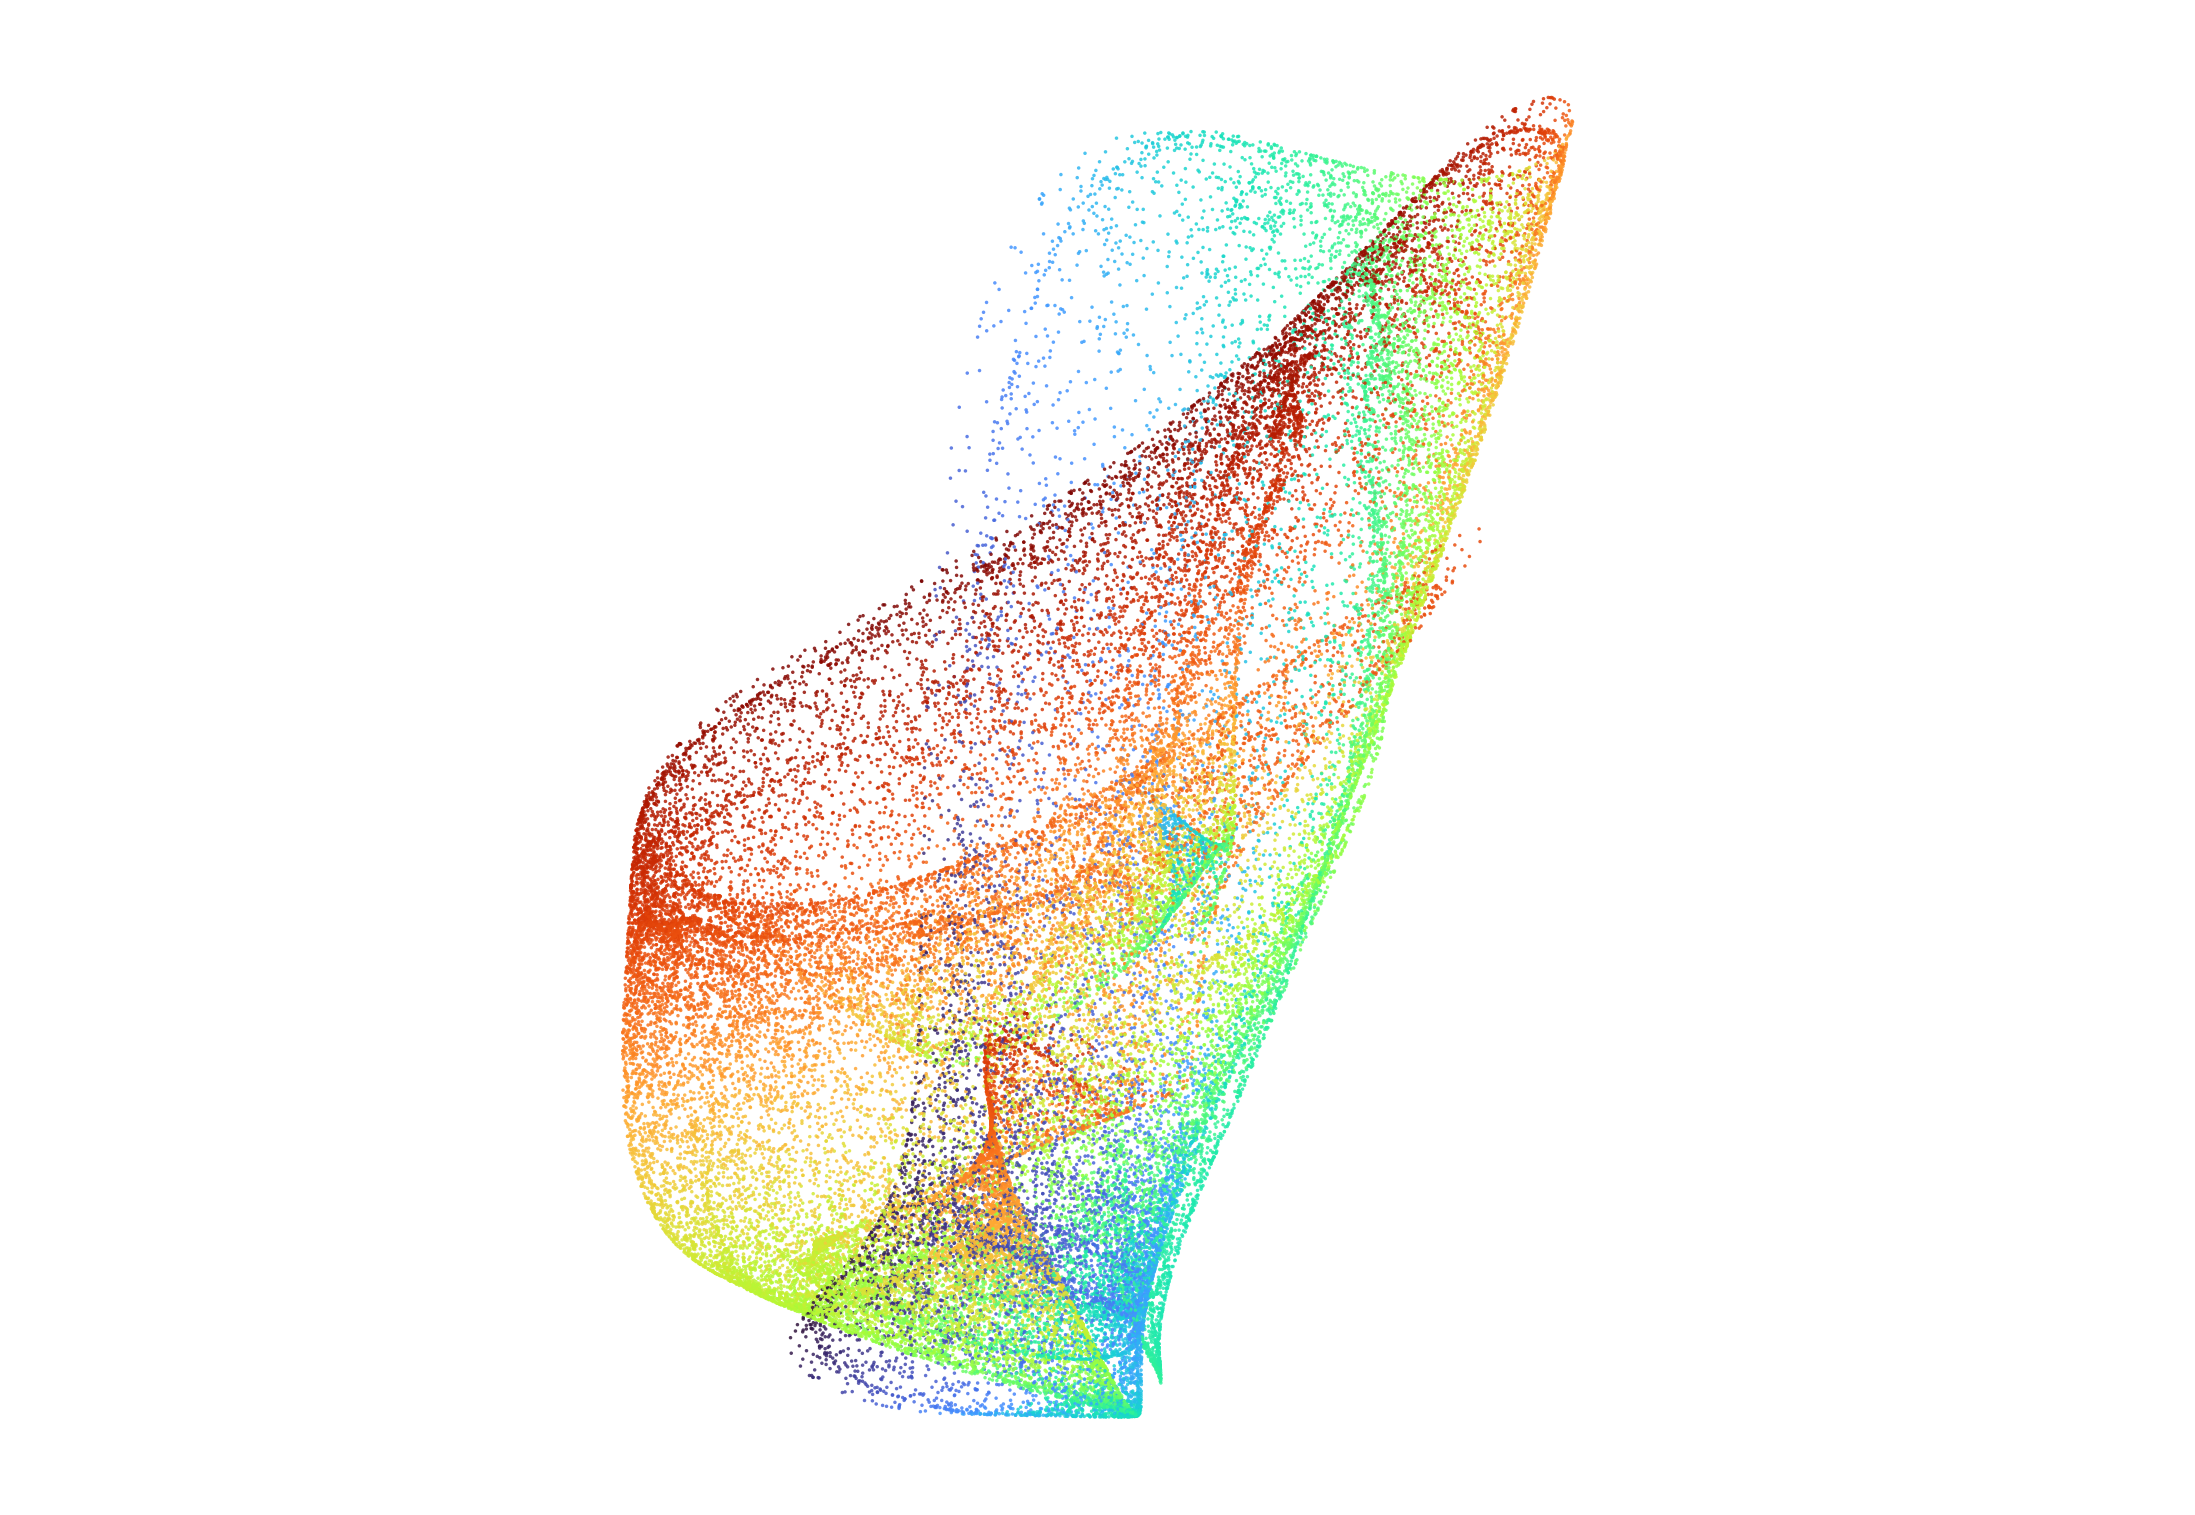
\includegraphics[width=0.60\linewidth]{sprott_map4d_turbo_white.png}
\caption{Ejemplo sintético público de una proyección \(x\)-\(y\) de un mapa 4D, con una paleta continua gobernada por \(w\). El color y la proyección son decisiones de visualización que deben registrarse junto con el código.}
\end{figure}
\thispagestyle{fancy}

Los archivos históricos de Sprott, sus figuras, ejecutables y diccionarios originales se consultan desde las páginas oficiales. La persona usuaria puede cargar localmente sus propios archivos \archivo{.DIC}; la aplicación los lee en su ubicación de origen.

La página del libro es \urlimpresa{https://sprott.physics.wisc.edu/SA.HTM} y el manuscrito en línea se encuentra en \urlimpresa{https://sprott.physics.wisc.edu/fractals/booktext/SABOOK.HTM}. El paquete editorial del disco puede consultarse en \urlimpresa{https://sprott.physics.wisc.edu/fractals/bookdisk/SADISK.ZIP}; su directorio oficial es \urlimpresa{https://sprott.physics.wisc.edu/fractals/bookdisk/}.

Para aprender la gramática, el fundamento algebraico de las familias, el significado de los filtros y el modo de lectura del libro, continúe en el \manualsprott.

\paragraph{Consulta de manuales en la aplicación.}

\campo{Manuales} reúne tres subpestañas. \campo{Usuario} abre este manual de operación; \campo{Teoría y diccionario} presenta la secuencia formativa de conceptos, definiciones, ecuaciones e interpretación de gráficas; y \campo{Explorador Sprott} abre el manual especializado en códigos compactos, simulación y lectura del libro. Esta organización permite consultar el nivel de explicación requerido sin salir de la aplicación. Los mismos documentos pueden abrirse como archivos independientes mediante el \manualteorico y el \manualsprott.

El menú \campo{Ayuda} reúne \boton{Documentacion}, que abre directamente el Manual de usuario; \boton{Buscar actualizaciones}, que realiza una comprobación manual cuando existe una fuente configurada; \boton{Revisar actualizaciones automaticamente}, que controla la comprobación periódica; y \boton{Acerca de}, donde se muestran versión, autoría, licencia y créditos de dependencias. Los otros dos documentos se eligen en la pestaña \campo{Manuales}. En \campo{Archivo}, \boton{Abrir carpeta de resultados} abre la ubicación predeterminada de resultados del usuario.

% Módulo sin preámbulo para manual_usuario_toolbox_chaos.tex.
% Contraste funcional: SYSTEM_REGISTRY, SystemParameterPanel, tab_controls,
% custom_system_tab y sprott_explorer_tab del árbol local de Toolbox Chaos.

\section{Protocolos de simulación y registro experimental}
\label{sec:recetario-ampliado}

Este recetario convierte una secuencia de controles en un experimento que otra
persona puede repetir. Cada receta separa siete componentes: la pregunta, el
modelo y sus valores exactos, la ruta por la interfaz, la salida esperada, la
lectura de la gráfica, una prueba de refinamiento y el límite de la evidencia.
El orden organiza la procedencia del experimento. Cuando se guarda primero una imagen y se reconstruye el
contrato después, es fácil omitir el estado inicial, el transitorio o una
decisión de muestreo que cambió el resultado.

Los nombres de pestañas y campos se reproducen literalmente y se destacan
tipográficamente; las acciones visibles se presentan como botones. Los valores
indicados pertenecen a la implementación actual. Al trabajar con otra versión,
anote cualquier diferencia en la bitácora en vez de ajustar silenciosamente el
protocolo.

\begin{cajaazul}{Regla de trabajo para todo el recetario}
Asigne un identificador a la corrida antes de calcular, cambie una sola familia
de controles durante la prueba de refinamiento y conserve por separado la
salida base y la refinada. En las pestañas generales, \boton{Guardar gráfica...}
guarda la figura. Complete también la plantilla de bitácora con todos los
parámetros de la
sección~\ref{sec:bitacora-reproducible}.
\end{cajaazul}

\subsection{Funciones de las trece pestañas}

La tabla siguiente permite elegir la herramienta por la pregunta que se desea
responder. También señala el límite operativo que debe quedar escrito en el
informe.

\begin{longtable}{@{}>{\raggedright\arraybackslash}p{0.16\linewidth}>{\raggedright\arraybackslash}p{0.22\linewidth}>{\raggedright\arraybackslash}p{0.24\linewidth}>{\raggedright\arraybackslash}p{0.22\linewidth}@{}}
\toprule
Pestaña & Pregunta operativa & Acción o producto principal & Límite que debe registrarse \\
\midrule
\endhead
\campo{Atractor 3D} & ¿Qué geometría muestra una trayectoria de tres componentes? & \boton{Generar atractor 3D} y \boton{Guardar gráfica...}. & El análisis de caos, atracción y estabilidad numérica requiere diagnósticos complementarios. \\
\campo{Retratos 2D} & ¿Qué estructura conservan las proyecciones por pares? & Simulación local o \boton{Usar última trayectoria}; panel de proyecciones. & Una proyección puede superponer estados distintos y ocultar otras coordenadas. \\
\campo{Series temporales} & ¿Cómo cambian las variables con el tiempo o la iteración? & Simulación local o reutilización de la última trayectoria. & La ventana finita puede mezclar transitorio y régimen posterior. \\
\campo{Comparar metodos} & ¿Qué cambia al usar Euler, Heun o RK4 con el mismo paso? & \boton{Comparar integradores}. & En caos, compare escala global, estructura de fase y diagnósticos declarados durante tiempos largos. \\
\campo{Espectro} & ¿Qué bandas o frecuencias aparecen en la muestra? & \campo{PSD de Welch (recomendado)} o \campo{Espectro de amplitud}. & Los máximos dependen del transitorio, la duración y la frecuencia de muestreo. \\
\campo{Lyapunov} & ¿Cómo evolucionan estimaciones finitas de separación local? & Espectro QR--Benettin con RK4 fijo. & Admite flujos ODE enteros registrados de tres dimensiones; una conclusión requiere la secuencia de refinamiento y convergencia del signo. \\
\campo{Bifurcación} & ¿Cómo cambia una observable al barrer un parámetro? & Barrido con transitorio, ventana útil y continuación opcional. & La resolución, el sentido del barrido y la clasificación numérica condicionan la figura. \\
\campo{Cuenca de atracción} & ¿Qué destino calcula cada condición inicial de una malla? & Clasificación en el plano \((x_0,y_0)\) con \(z_0\) fijo. & La certificación de destinos globales y fronteras exactas requiere análisis de cobertura y convergencia. \\
\campo{Autovalores} & ¿Qué predice la linealización cerca de un equilibrio? & Equilibrios y autovalores en el plano complejo. & La dinámica alejada del equilibrio requiere trayectorias, cuencas y análisis globales complementarios. \\
\campo{Coexistencia} & ¿Qué ocurre con varias condiciones iniciales y los mismos parámetros? & Simulación de uno o todos los casos catalogados. & La clasificación de los destinos posibles requiere una cobertura de condiciones iniciales y sus diagnósticos. \\
\campo{Manuales} & ¿Qué fundamento o procedimiento hace falta consultar? & Tres manuales integrados: usuario, teoría y Explorador Sprott. & El registro de la corrida concreta aporta la procedencia experimental. \\
\campo{Crear sistema} & ¿Qué trayectoria produce una definición algebraica propia? & Validación restringida, simulación y archivo JSON. & Equilibrios, Jacobiano, caos, atracción global y cuencas requieren los flujos de análisis y curación correspondientes. \\
\campo{Explorador Sprott} & ¿Qué sistema representa un código compacto y cómo se explora? & Decodificación, simulación, búsqueda, estilo, galería y exportaciones. & Los filtros rápidos producen candidatos; la certificación de caos o atracción requiere diagnósticos adicionales. \\
\bottomrule
\end{longtable}

\subsection{Protocolo 1. Trayectoria de Lorenz en varias pestañas}

\begin{cajaazul}{Trayectoria de Lorenz y diagnósticos}
¿La geometría de dos lóbulos, la irregularidad temporal, el contenido espectral
y la estimación de Lyapunov describen de manera compatible una misma corrida de
Lorenz?
\end{cajaazul}

\paragraph{Parámetros de Lorenz.}
Use \campo{Lorenz [listo]}, \(\sigma=10\), \(\rho=28\),
\(\beta=2.666667\), \(x(0)=y(0)=z(0)=0.1\),
\campo{Runge--Kutta 4 [C]}, \campo{dt}=0.01 y
\campo{Tiempo total T}=40. Para la PSD descarte 5 unidades de tiempo y deje
ambos límites de frecuencia en cero. Para Lyapunov use
\campo{dt integrador}=0.01, \campo{Burn-in time}=5,
\campo{Tiempo final}=40 y \campo{QR cada N pasos}=10.

\paragraph{Controles de la simulación.}
\begin{enumerate}
  \item Abra \campo{Atractor 3D}, capture el contrato anterior y pulse
  \boton{Generar atractor 3D}. Guarde la figura como
  \archivo{r01_lorenz_atractor_base.png}.
  \item Abra \campo{Retratos 2D}, seleccione también
  \campo{Lorenz [listo]} y pulse \boton{Usar última trayectoria}. Conserve los
  planos \(x\)-\(y\), \(x\)-\(z\) y \(y\)-\(z\); guarde
  \archivo{r01_lorenz_retratos_base.png}.
  \item En \campo{Series temporales}, seleccione Lorenz y pulse
  \boton{Usar última trayectoria}. Guarde
  \archivo{r01_lorenz_series_base.png}.
  \item En \campo{Espectro}, seleccione
  \campo{PSD de Welch (recomendado)}, escriba 5 en
  \campo{Descartar transitorio (s)}, deje los límites automáticos en cero y
  pulse \boton{Usar última trayectoria}. Guarde
  \archivo{r01_lorenz_psd_base.png}.
  \item En \campo{Lyapunov}, seleccione Lorenz, capture los cuatro valores
  indicados, pulse \boton{Calcular exponentes de Lyapunov} y guarde
  \archivo{r01_lorenz_lyapunov_base.png}.
\end{enumerate}

\begin{cajaverde}{Geometría, series y Lyapunov de Lorenz}
La vista 3D debe organizarse alrededor de dos lóbulos; los retratos 2D muestran
proyecciones diferentes de los mismos estados y las series alternan episodios
asociados a ambos lóbulos. Una PSD distribuida en varias frecuencias es
compatible con una señal de varias componentes o con modulación irregular. En Lyapunov importa la curva
de convergencia además del valor final: registre los tres exponentes mostrados
y si el máximo conserva su signo durante la parte tardía de la ventana.
\end{cajaverde}

\figuradidactica{systems/lorenz_phase_timeseries.png}{Lectura conjunta de Lorenz: la geometría tridimensional identifica los dos lóbulos y las series temporales muestran cuándo la trayectoria cambia de uno a otro. Los ejes y el pie contienen la información descriptiva y mantienen una composición gráfica limpia.}

\paragraph{Refinamiento del paso temporal.}
Repita la trayectoria con \campo{dt}=0.005 y \campo{Tiempo total T}=40;
regenere las tres representaciones desde esa nueva corrida. Para Lyapunov use
\campo{dt integrador}=0.005, \campo{Burn-in time}=5,
\campo{Tiempo final}=80 y \campo{QR cada N pasos}=10. Compare extensión,
rangos, lóbulos, bandas espectrales y tendencia de los exponentes. Use esos
indicadores para comparar las trayectorias tardías.

\begin{cajaalerta}{Diagnósticos para caos y atracción en Lorenz}
La identificación de caos y atracción requiere varios diagnósticos. La forma de mariposa y una PSD ancha orientan el análisis, mientras que un exponente máximo positivo aporta evidencia numérica dentro del
contrato usado. Una demostración matemática y la convergencia entre plataformas
requieren sus desarrollos y verificaciones correspondientes.
\end{cajaalerta}

\paragraph{Archivos y metadatos de Lorenz.}
Conserve las cinco figuras base, sus versiones con sufijo
\archivo{_dt0005}, y \archivo{r01_lorenz_bitacora.txt}. En la bitácora anote
versión, plataforma, parámetros, estado inicial, método, ambos pasos, tiempos,
transitorio de la PSD, controles de Lyapunov, nombres de salida y los valores
numéricos reportados por la interfaz.

\subsection{Protocolo 2. Mapa logístico y diagrama de bifurcación}

\begin{cajaazul}{Bifurcaciones del mapa logístico}
¿Qué cambios cualitativos aparecen en los valores tardíos de
\(x_{n+1}=r x_n(1-x_n)\) cuando \(r\) recorre el intervalo de 2.5 a 4.0?
\end{cajaazul}

\paragraph{Parámetros del mapa logístico.}
En \campo{Bifurcación} seleccione \campo{Logistico [listo]},
\(x(0)=0.2\), \campo{Parámetro de bifurcación}=\campo{r},
\campo{Variable observada}=\campo{x}, \campo{Mínimo}=2.5,
\campo{Máximo}=4.0, \campo{N (Parámetros)}=350,
\campo{dt integrador}=1, \campo{Transitorio descartado}=600,
\campo{Tiempo útil}=500 y \campo{Máx cruces por param}=250.
Mantenga desactivado \campo{Usar continuación} en la corrida base.

\paragraph{Controles del diagrama de bifurcación.}
\begin{enumerate}
  \item Confirme que el selector del mapa deshabilita el integrador: una
  iteración pertenece al modelo; el paso temporal corresponde a una EDO.
  \item Capture los valores del barrido y pulse
  \boton{Calcular bifurcación}.
  \item Lea primero el eje horizontal y confirme que cubre 2.5--4.0; después
  examine cuántos valores tardíos aparecen para cada parámetro.
  \item Guarde \archivo{r02_logistico_bif_base.png}.
\end{enumerate}

\begin{cajaverde}{Ramas y bandas del mapa logístico}
La figura debe pasar de una rama a duplicaciones sucesivas, regiones densas y
ventanas más ordenadas. Una columna representa una muestra tardía para un valor
de \(r\); su densidad vertical registra la multiplicidad de valores y puede estar limitada por
\campo{Máx cruces por param}. Distinga una ventana visible de la afirmación de
que se conoce su periodo exacto.
\end{cajaverde}

\figuradidactica{logistic_bifurcation.png}{Barrido reproducible del mapa logístico. Una sola altura por parámetro indica un estado asintótico fijo; dos, cuatro y más alturas revelan duplicaciones de periodo; las bandas densas deben contrastarse con series y refinamiento.}

\paragraph{Resolución del barrido paramétrico.}
Repita sin continuación con \campo{N (Parámetros)}=700,
\campo{Transitorio descartado}=1000, \campo{Tiempo útil}=800 y
\campo{Máx cruces por param}=500. Guarde
\archivo{r02_logistico_bif_refinada.png}. Después, si desea estudiar dependencia
de rama, active \campo{Usar continuación} y guarde esa corrida con el sufijo
\archivo{_continuacion}; manténgala como una corrida separada de la prueba de resolución.

\begin{cajaalerta}{Resolución y parámetros críticos del mapa logístico}
La caracterización de cada banda y la localización de parámetros críticos requieren
resolver el barrido con precisión suficiente. La resolución horizontal, el
transitorio y la cantidad de valores guardados condicionan las estructuras
pequeñas.
\end{cajaalerta}

\paragraph{Archivos y metadatos del mapa logístico.}
Guarde las dos figuras principales, la comparación opcional de continuación y
\archivo{r02_logistico_bitacora.txt}. Registre ecuación, \(x(0)\), intervalo,
número de parámetros, transitorio, ventana útil, límite por columna, estado de
continuación y dirección del barrido.

\subsection{Protocolo 3. Mapa de Hénon y retrato de fase}

\begin{cajaazul}{Retrato de fase del mapa de Hénon}
¿Cómo se organiza en el plano \(x\)-\(y\) la órbita del mapa de Hénon y qué
aspectos permanecen al aumentar el número de iteraciones?
\end{cajaazul}

\paragraph{Parámetros del mapa de Hénon.}
Use \campo{Henon [listo]}, \(a=1.4\), \(b=0.3\),
\(x(0)=0.1\), \(y(0)=0.1\), \campo{dt}=1 y
\campo{Tiempo total T}=5000. El campo de método debe quedar deshabilitado por
tratarse de un mapa. El estado 2D queda definido por las dos primeras condiciones iniciales.

\paragraph{Controles de iteración y retrato.}
\begin{enumerate}
  \item Abra \campo{Retratos 2D}, seleccione Hénon y confirme los valores.
  \item En \campo{Proyecciones 2D}, conserve \campo{Plano x-y}.
  \item Pulse \boton{Generar retratos 2D} y guarde
  \archivo{r03_henon_xy_base.png}.
  \item Abra \campo{Series temporales}, seleccione Hénon y pulse
  \boton{Usar última trayectoria}; guarde
  \archivo{r03_henon_series_base.png}.
\end{enumerate}

\begin{cajaverde}{Geometría plegada e iteraciones de Hénon}
El plano debe mostrar un conjunto plegado y delgado, con estructura distinta de una curva
cerrada simple. Las series de \(x_n\) y \(y_n\) permiten comprobar que cada
punto procede de la iteración anterior. La pestaña 3D trabaja con tres
coordenadas, mientras este sistema registra dimensión dos; use el plano \(x\)-\(y\).
\end{cajaverde}

\figuradidactica{systems/henon_phase_timeseries.png}{El retrato de Hénon conserva la geometría de las iteraciones después del transitorio, mientras las series separan el orden temporal que se pierde en la nube del plano.}

\paragraph{Longitud de la iteración.}
En un mapa, refine la longitud de la iteración. Repita con
\campo{Tiempo total T}=10000 y los demás valores intactos. Compare el soporte,
los rangos y las zonas de mayor densidad visual. Como prueba separada de
sensibilidad, use \(x(0)=0.100001\), \(y(0)=0.1\); etiquete esa salida como
perturbación inicial y regístrela como una prueba de sensibilidad distinta del refinamiento temporal.

\begin{cajaalerta}{Diagnósticos de invariancia y caos en Hénon}
La forma plegada aporta geometría proyectada. La dimensión fractal, la ergodicidad,
la invariancia y el caos requieren sus diagnósticos correspondientes. El panel incluye el arranque de la órbita; registre el intervalo de análisis seleccionado para la interpretación posterior.
\end{cajaalerta}

\paragraph{Archivos y metadatos del mapa de Hénon.}
Conserve \archivo{r03_henon_xy_base.png},
\archivo{r03_henon_xy_n10000.png}, las series y, si se ejecutó, la perturbación.
Registre que \(T\) se interpreta como número de iteraciones porque \(dt=1\),
además de parámetros, estado inicial y cantidad total de puntos.

\subsection{Protocolo 4. Sistema de Rössler e integradores}

\begin{cajaazul}{Sensibilidad numérica del sistema de Rössler}
¿Qué rasgos globales del flujo de Rössler son estables frente a Euler, Heun y
RK4, y en qué momento dejan de coincidir sus trayectorias?
\end{cajaazul}

\paragraph{Parámetros del sistema de Rössler.}
En \campo{Comparar metodos} seleccione \campo{Rossler [listo]},
\(a=0.2\), \(b=0.2\), \(c=5.7\),
\((x(0),y(0),z(0))=(0.1,0,0)\), \campo{dt}=0.01 y
\campo{Tiempo total T}=80. Active \campo{Euler explícito},
\campo{Heun / Euler mejorado (RK2)} y \campo{Runge--Kutta 4}; asigne un color
distinto a cada método.

\paragraph{Controles de integración.}
\begin{enumerate}
  \item Confirme que los tres integradores están activos y pulse
  \boton{Comparar integradores}.
  \item Guarde \archivo{r04_rossler_metodos_dt001.png}.
  \item Abra \campo{Retratos 2D}, capture el mismo modelo con
  \campo{Runge--Kutta 4 [C]}, \(dt=0.01\), \(T=80\), genere los retratos y
  guarde \archivo{r04_rossler_retratos_rk4.png}.
\end{enumerate}

\begin{cajaverde}{Trayectorias e integradores de Rössler}
Las series deben mostrar oscilaciones que crecen alrededor de una región y una
excursión de retorno; en el plano aparece la geometría espiral característica.
Las curvas pueden separarse en fase con el tiempo. Compare amplitudes, rangos,
periodo aproximado de las vueltas y presencia de la excursión, junto con
la convergencia de las propiedades reportadas.
\end{cajaverde}

\figuradidactica{systems/rossler_phase_timeseries.png}{Rössler en espacio de fases y en el tiempo. La espiral casi plana explica por qué distintas proyecciones pueden parecer regulares aunque las excursiones de la tercera coordenada introduzcan otra escala dinámica.}

\paragraph{Convergencia al reducir el paso.}
Repita la comparación con \campo{dt}=0.005 y \campo{Tiempo total T}=80.
Guarde \archivo{r04_rossler_metodos_dt0005.png}. Compruebe si Heun y RK4
conservan durante más tiempo la escala y la fase, y registre si Euler presenta
sesgo o inestabilidad. Conserve cada salida inesperada como parte del
diagnóstico.

\begin{cajaalerta}{Convergencia de los integradores de Rössler}
La estimación del error global requiere comparar cuantitativamente los métodos y sus
refinamientos. Una divergencia tardía orienta la revisión del horizonte y del paso. Hace falta
una secuencia de pasos y observables cuantitativas para sostener convergencia.
\end{cajaalerta}

\paragraph{Archivos y metadatos de Rössler.}
Guarde las dos comparaciones, el retrato RK4 y
\archivo{r04_rossler_bitacora.txt}. Anote versión, ecuaciones de referencia,
parámetros, estado inicial, métodos activados, colores, pasos, horizonte y el
primer intervalo temporal en que las curvas dejan de ser visualmente próximas.

\subsection{Protocolo 5. Circuito de Chua y condición inicial}

\begin{cajaazul}{Condiciones iniciales y simetría de Chua}
¿Dos condiciones iniciales simétricas, con exactamente los mismos parámetros de
Chua, producen trayectorias reflejadas y una geometría de doble scroll durante
el horizonte simulado?
\end{cajaazul}

\paragraph{Parámetros del circuito de Chua.}
En \campo{Atractor 3D} elija \campo{Chua}. Use
\(\alpha=15.6\), \(\beta=28\), \(m_0=-1.143\), \(m_1=-0.714\), con
\((0.1,0,0)\) en la primera corrida y \((-0.1,0,0)\) en la segunda.
Seleccione RK4, \campo{dt}=0.01 y \campo{Tiempo T}=80.

\paragraph{Controles de la simulación de Chua.}
\begin{enumerate}
  \item Introduzca los parámetros y la condición inicial \((0.1,0,0)\), pulse
  \boton{Generar atractor 3D} y guarde \archivo{r05_chua_ic_positiva.png}.
  \item Cambie únicamente la condición inicial a \((-0.1,0,0)\), repita la
  simulación y guarde \archivo{r05_chua_ic_negativa.png}.
  \item Abra \campo{Series temporales} y conserve las componentes de ambas
  corridas con nombres que identifiquen claramente el signo del inicio.
  \item Compare \((x,y,z)\) de una corrida con \((-x,-y,-z)\) de la otra. La
  simetría del campo vectorial permite comprobar numéricamente el reflejo sin
  confundirlo con dos sistemas diferentes.
\end{enumerate}

\begin{cajaverde}{Simetría numérica en las trayectorias de Chua}
Las dos corridas deben ser finitas, recorrer una geometría de doble scroll y
aparecer como reflejos dentro del error numérico. Lea la comparación como una
verificación de simetría y de sensibilidad de la trayectoria concreta al signo
del inicio. La existencia de dos destinos asintóticos distintos requiere una
exploración de cuencas y condiciones iniciales.
\end{cajaverde}

\figuradidactica{systems/chua_phase_timeseries.png}{Chua con trayectoria tridimensional y componentes temporales. La figura permite comprobar doble scroll, finitud y escalas; la pareja de condiciones iniciales de la receta debe analizarse además mediante el error de simetría.}

\paragraph{Sensibilidad a la condición inicial.}
Repita ambas corridas con \campo{dt}=0.005 y \campo{Tiempo T}=80. Después
ejecute una tercera pareja con \campo{dt}=0.01 y \campo{Tiempo T}=160 para
separar el efecto del paso del efecto del horizonte. Compare la región visitada,
la simetría y las estadísticas globales como criterios de comparación a tiempos
tardíos.

\begin{cajaalerta}{Cuencas y coexistencia en el circuito de Chua}
Esta reproducción muestra dos trayectorias simétricas para el protocolo
declarado. La caracterización de caos, coexistencia de destinos asintóticos y fronteras de cuencas requiere ampliar las condiciones iniciales y los diagnósticos.
\end{cajaalerta}

\paragraph{Archivos y metadatos de Chua.}
Conserve las figuras y series de las dos corridas, las pruebas de refinamiento y
\archivo{r05_chua_bitacora.txt}. Incluya parámetros, ambas condiciones
iniciales, método, \(dt\), \(T\), norma del error de simetría y nombres de
archivo.

\subsection{Protocolo 6. Duffing--Ueda y muestreo del forzamiento}

\begin{cajaazul}{Muestreo del forzamiento Duffing--Ueda}
¿El paso temporal resuelve suficientemente el periodo del forzamiento y se
conservan la envolvente y las bandas espectrales de la respuesta Duffing--Ueda?
\end{cajaazul}

\paragraph{Parámetros de Duffing--Ueda.}
En \campo{Series temporales} seleccione \campo{Duffing-Ueda [listo]},
\(\delta=0.2\), \(\alpha=-1\), \(\beta=1\), \(\gamma=0.3\),
\(\omega=1.2\), \((x(0),y(0),\theta(0))=(0.1,0,0)\),
\campo{Runge--Kutta 4 [C]}, \campo{dt}=0.01 y
\campo{Tiempo total T}=200. El periodo de forzamiento es
\[
  P_f=\frac{2\pi}{\omega}=5.235988\ldots,
\]
por lo que la malla base contiene aproximadamente 523.6 muestras por periodo.

\paragraph{Controles de integración y muestreo.}
\begin{enumerate}
  \item Pulse \boton{Generar series temporales} y guarde
  \archivo{r06_duffing_series_dt001.png}.
  \item Abra \campo{Retratos 2D}, seleccione Duffing--Ueda y pulse
  \boton{Usar última trayectoria}. Conserve el plano \(x\)-\(y\) y guarde
  \archivo{r06_duffing_xy_dt001.png}.
  \item Abra \campo{Espectro}, seleccione
  \campo{PSD de Welch (recomendado)}, escriba 50 en
  \campo{Descartar transitorio (s)}, deje los límites de frecuencia en cero y
  pulse \boton{Usar última trayectoria}. Guarde
  \archivo{r06_duffing_psd_dt001.png}.
\end{enumerate}

\begin{cajaverde}{Respuesta temporal y espectral de Duffing--Ueda}
La tercera variable debe crecer como fase extendida porque
\(\dot\theta=\omega\); la fuerza usa \(\cos\theta\), de modo que el fenómeno
físico asociado sigue siendo periódico. Lea en \(x(t)\) y \(y(t)\) la amplitud,
los cambios de pozo y la regularidad de los ciclos. En la PSD, la frecuencia de
forzamiento en ciclos por unidad de tiempo es
\(f_f=\omega/(2\pi)\approx0.190986\); anote bandas cercanas y sus armónicos sin
suponer que todo máximo procede directamente del forzamiento.
\end{cajaverde}

\figuradidactica{systems/duffing_ueda_phase_timeseries.png}{Respuesta forzada de Duffing--Ueda. El retrato proyectado resume la región visitada y las series permiten reconocer el periodo del forzamiento, el transitorio y los cambios al refinar el paso.}

\paragraph{Resolución temporal del forzamiento.}
Repita con \campo{dt}=0.005 y \campo{Tiempo total T}=200; ahora hay unas
1047.2 muestras por periodo. Mantenga el mismo descarte de 50 y compare rangos,
envolvente del plano \(x\)-\(y\) y posiciones de los máximos espectrales. La
interfaz general analiza las series temporales directamente. Una sección de
Poincaré requiere un muestreo estroboscópico dedicado, una vez por periodo.

\begin{cajaalerta}{Caos y convergencia en Duffing--Ueda}
Resolver el forzamiento con muchas muestras permite estudiar la respuesta temporal; el caos y la convergencia global requieren diagnósticos adicionales. Una rampa de \(\theta\) corresponde al avance de fase del forzamiento y
la fase extendida que usa la formulación autónoma correspondiente.
\end{cajaalerta}

\paragraph{Archivos y metadatos de Duffing--Ueda.}
Guarde las seis figuras base/refinadas y
\archivo{r06_duffing_muestreo.txt}. Registre \(P_f\), \(f_f\), muestras por
periodo, parámetros, estado inicial, método, paso, horizonte, transitorio de la
PSD y si se observaron cambios de pozo.

\subsection{Protocolo 7. Mackey--Glass e historia retardada}

\begin{cajaazul}{Historia retardada de Mackey--Glass}
¿La oscilación de Mackey--Glass y su contenido espectral permanecen al refinar
la interpolación temporal de una historia con retardo \(\tau=17\)?
\end{cajaazul}

\paragraph{Parámetros de Mackey--Glass.}
En \campo{Series temporales} seleccione \campo{Mackey-Glass [listo]},
\(\beta=0.2\), \(\gamma=0.1\), \(n=10\), \(\tau=17\),
\(x(0)=1.2\), \campo{Runge--Kutta 4 [C]}, \campo{dt}=0.1 y
\campo{Tiempo total T}=500. Deje en cero los dos campos iniciales mostrados con
guion: el backend construye la historia previa como constante igual a
\(x(0)\). Para RK4 usa interpolación cúbica causal por tramos.

\paragraph{Controles de historia y ventana.}
\begin{enumerate}
  \item Pulse \boton{Generar series temporales} y guarde
  \archivo{r07_mackey_series_dt01.png}.
  \item Identifique los tres canales devueltos por la implementación: valor
  actual, valor retardado y derivada. Los guiones de la interfaz identifican
  los campos de una historia con retardo.
  \item Abra \campo{Espectro}, seleccione
  \campo{PSD de Welch (recomendado)}, establezca
  \campo{Descartar transitorio (s)}=100, deje los límites automáticos y pulse
  \boton{Usar última trayectoria}. Guarde
  \archivo{r07_mackey_psd_dt01.png}.
\end{enumerate}

\begin{cajaverde}{Canales temporales y espectro de Mackey--Glass}
Después de la historia inicial deben aparecer oscilaciones acotadas cuya
amplitud y separación entre máximos pueden variar. Compare el canal actual con
el retardado para reconocer el desplazamiento de \(\tau\). La PSD resume la
ventana posterior a \(t=100\); el análisis de la ecuación diferencial funcional complementa las bandas.
\end{cajaverde}

\figuradidactica{systems/mackey_glass_phase_timeseries.png}{Mackey--Glass requiere leer una ventana larga: la proyección organiza estados retardados y la serie temporal muestra si el horizonte contiene suficientes oscilaciones para sostener la interpretación.}

\paragraph{Longitud de la ventana de observación.}
Repita con \campo{dt}=0.05 y \campo{Tiempo total T}=500, sin cambiar historia,
parámetros ni método. Vuelva a descartar 100 en la PSD. Compare rangos, tiempos
aproximados de máximos y ubicación de bandas. Si difieren materialmente, pruebe
\(dt=0.025\) antes de interpretar la corrida.

\begin{cajaalerta}{Diagnósticos de historias y atracción en Mackey--Glass}
Una señal irregular requiere diagnósticos de caos en el espacio de historias, y la atracción global exige explorar varias historias iniciales. La representación de tres canales es
una vista de una dinámica con memoria; la EDO autónoma tridimensional ordinaria
requiere una formulación de estado distinta.
\end{cajaalerta}

\paragraph{Archivos y metadatos de Mackey--Glass.}
Conserve las series y PSD para ambos pasos y
\archivo{r07_mackey_bitacora.txt}. Incluya la historia constante, \(x(0)\),
\(\beta,\gamma,n,\tau\), interpolación asociada a RK4, pasos, horizonte,
transitorio, versión y cualquier advertencia de memoria o no finitud.

\subsection{Protocolo 8. Lorenz--96 y proyecciones de ocho variables}

\begin{cajaazul}{Proyecciones de ocho variables de Lorenz--96}
¿Qué evolución muestran las tres primeras componentes de Lorenz--96 cuando una
perturbación pequeña rompe el estado uniforme de un anillo con \(J=8\)?
\end{cajaazul}

\paragraph{Parámetros de Lorenz--96.}
Use \campo{Lorenz-96 [listo]}, \(F=8\), \(J=8\),
\((X_1(0),X_2(0),X_3(0))=(8.01,8,8)\),
\campo{Runge--Kutta 4 [C]}, \campo{dt}=0.01 y
\campo{Tiempo total T}=40. El backend inicializa las restantes componentes del
anillo con \(F\) y devuelve a la interfaz sólo \(X_1,X_2,X_3\).

\paragraph{Controles de la proyección.}
\begin{enumerate}
  \item Abra \campo{Atractor 3D}, capture los valores y pulse
  \boton{Generar atractor 3D}. Guarde
  \archivo{r08_lorenz96_proyeccion3d_base.png}.
  \item Abra \campo{Retratos 2D}, seleccione Lorenz--96 y pulse
  \boton{Usar última trayectoria}. Guarde
  \archivo{r08_lorenz96_retratos_base.png}.
  \item En \campo{Series temporales}, seleccione Lorenz--96, pulse
  \boton{Usar última trayectoria} y guarde
  \archivo{r08_lorenz96_series_base.png}.
\end{enumerate}

\begin{cajaverde}{Propagación y proyecciones de Lorenz--96}
La perturbación inicial debe propagarse y las tres componentes mostradas dejan
de permanecer exactamente en el nivel uniforme. Lea la vista 3D y los planos
como proyecciones de una trayectoria de ocho variables. La cercanía o cruce de
dos puntos en \((X_1,X_2,X_3)\) aportan una coincidencia proyectada; la igualdad
del estado completo requiere comparar las ocho componentes.
\end{cajaverde}

\figuradidactica{systems/lorenz96_phase_timeseries.png}{Proyección de Lorenz--96. La salida gráfica actual muestra tres componentes; el pie recuerda que el estado integrado contiene ocho variables y presenta una vista parcial del sistema completo.}

\paragraph{Selección de componentes observadas.}
Repita con \campo{dt}=0.005 y \campo{Tiempo total T}=40. Compare rangos,
estructura proyectada y escalas temporales. Como experimento distinto del
refinamiento, puede cambiar \(J\); tal cambio modifica la dimensión del modelo
y requiere una nueva bitácora.

\begin{cajaalerta}{Transporte y extensividad en Lorenz--96}
La proyección de tres componentes describe una vista parcial del estado de
Lorenz--96. El transporte en el anillo y la extensividad del caos requieren cálculos específicos. La etiqueta ``atractor 3D'' se reserva para la
ocho.
\end{cajaalerta}

\paragraph{Archivos y metadatos de Lorenz--96.}
Guarde las seis figuras base/refinadas y
\archivo{r08_lorenz96_bitacora.txt}. Registre \(F\), \(J\), las tres entradas
visibles, la regla de inicialización de las cinco restantes, método, paso,
horizonte y las coordenadas proyectadas.

\subsection{Protocolo 9. Genesio--Tesi en Crear sistema}

\begin{cajaazul}{Definición de Genesio--Tesi en el editor}
¿Puede el editor restringido validar, simular y conservar una definición de
Genesio--Tesi sin ejecutar código Python arbitrario?
\end{cajaazul}

\paragraph{Ecuaciones y parámetros de Genesio--Tesi.}
En \campo{Crear sistema} capture los campos siguientes.

\begin{tabularx}{\linewidth}{>{\raggedright\arraybackslash}p{0.34\linewidth}X}
\toprule
Campo & Valor \\
\midrule
\campo{Nombre} & \archivo{Genesio-Tesi} \\
\campo{Tipo} & \campo{Flujo continuo} \\
\campo{Variables (separadas por coma)} & \archivo{x, y, z} \\
\campo{Parametros (nombre=valor)} & \archivo{a=1.2}, \archivo{b=2.92}, \archivo{c=6.0}, una asignación por línea \\
\campo{Ecuaciones (una por variable)} & \archivo{y}; \archivo{z}; \archivo{-c*x-b*y-a*z+x**2}, una expresión por línea \\
\campo{Estado inicial} & \archivo{0.2, 0.2, 0.2} \\
\campo{Metodo del flujo} & \archivo{rk4} \\
\campo{Paso h} & \archivo{0.005000} \\
\campo{Duracion} & \archivo{500.0000} \\
\campo{Muestras transitorias} & \archivo{5000} \\
\campo{Umbral de divergencia} & \archivo{1000000.00} \\
\bottomrule
\end{tabularx}

\paragraph{Controles de Crear sistema.}
\begin{enumerate}
  \item Pulse \boton{Validar definicion}. Exija el mensaje de definición válida
  antes de simular.
  \item Pulse \boton{Simular y graficar}. Registre estado, pasos completados,
  pasos solicitados y motor mostrado.
  \item Pulse \boton{Guardar JSON} y use el nombre
  \archivo{r09_genesio_tesi_definicion.json}.
  \item Abra \campo{Espectro}, fije
  \campo{PSD de Welch (recomendado)},
  \campo{Descartar transitorio (s)}=25 y pulse
  \boton{Usar última trayectoria}. Guarde
  \archivo{r09_genesio_tesi_psd_base.png}.
\end{enumerate}

\begin{cajaverde}{Trayectoria y PSD de Genesio--Tesi}
La validación debe reconocer tres variables y un flujo. La simulación debe
completar una trayectoria finita o informar explícitamente el punto de fallo.
El gráfico integrado muestra la proyección de las tres variables después de
retirar las muestras transitorias elegidas. El JSON conserva la definición
algebraica; la PSD permite revisar escalas de la trayectoria compartida.
\end{cajaverde}

\figuradidactica{variational_volume_manifolds.png}{Apoyo para interpretar un sistema personalizado: el campo determina la órbita, su variacional describe la deformación local y las direcciones estables e inestables organizan el movimiento próximo. La interpretación integra la simulación con esa lectura variacional.}

\paragraph{Verificación de la definición ingresada.}
Repita con \campo{Paso h}=0.002500, \campo{Duracion}=500 y
\campo{Muestras transitorias}=10000. El cambio de 5000 a 10000 mantiene en 25
unidades de tiempo el tramo retirado. Compare región visitada, rangos y PSD;
guarde la figura refinada con el sufijo \archivo{_h00025}.

\begin{cajaalerta}{Evidencia necesaria y alcance de la reutilización}
Una definición válida satisface el contrato sintáctico y numérico del
motor. La evaluación de caos y atracción global requiere diagnósticos posteriores. En la interfaz actual,
\campo{Retratos 2D} y \campo{Series temporales} comparan la clave de la última
trayectoria con el catálogo y pueden rechazar la clave personalizada. La ruta
verificada para reutilizarla es \campo{Espectro}. Registre la compatibilidad
mostrada por la interfaz antes de declarar la reutilización en los otros botones.
\end{cajaalerta}

\paragraph{Archivos y metadatos de Genesio--Tesi.}
Conserve el JSON, ambas PSD y \archivo{r09_genesio_tesi_bitacora.txt}. El JSON conserva la definición algebraica. Añada a la bitácora el paso, la duración,
las muestras transitorias, el umbral, la versión del motor, el estado y el conteo de pasos.

\subsection{Protocolo 10. Código Sprott y exportación}

\begin{cajaazul}{Código compacto y exportación de Sprott}
¿Puede reconstruirse un mapa 2D desde un código compacto y conservarse la
trayectoria separada de las decisiones de estilo?
\end{cajaazul}

\paragraph{Código y parámetros Sprott.}
Use el código \archivo{EWMWAMMMPMMMM}. En \campo{Exploracion} establezca
\campo{Tipo}=\archivo{map}, \campo{Dimension}=2, \campo{Orden}=2,
\campo{\mbox{Iteraciones}/\allowbreak\mbox{pasos}}=12000, \campo{Transitorio}=1500,
\campo{Tolerancia divergencia}=1000000, \campo{Semilla aleatoria}=1 y
\campo{Codigo}=\archivo{EWMWAMMMPMMMM}. Para un código fijo, semilla,
\campo{Paso h} y \campo{Metodo flujo} documentan el estado visible de esta interfaz; la iteración del mapa queda definida por el código, la semilla y los parámetros. Manténgalos
en 1, 0.01 y \archivo{rk4}.

Use además \campo{Proyeccion}=\archivo{x-y},
\campo{Color por}=\archivo{tiempo}, \campo{Paleta}=\campo{Viridis},
\campo{Fondo}=\campo{blanco}, \campo{Modo dibujo}=\campo{puntos},
\campo{Tamano punto}=0.70, \campo{Opacidad}=0.75,
\campo{Max puntos}=12000, \campo{Bandas}=0 y
\campo{DPI export}=220. Active \campo{Mostrar ejes},
\campo{Mostrar grid} y \campo{Aspect ratio igual}.

\paragraph{Controles de estilo y exportación.}
\begin{enumerate}
  \item En \campo{Codigos}, pegue el código y pulse \boton{Decodificar}.
  Verifique que las ecuaciones reconstruidas sean
  \[
    x_{n+1}=1+y_n-1.2x_n^2,
    \qquad y_{n+1}=0.3x_n.
  \]
  \item Pase a \campo{Exploracion}, capture el contrato anterior y pulse
  \boton{Simular y graficar}. Lea estado, razón y rangos antes de cambiar el
  estilo.
  \item Capture los controles visuales y pulse \boton{Aplicar estilo}. Cambiar
  estilo debe conservar la órbita almacenada y modificar únicamente su representación.
  \item Pulse \boton{Exportar imagen actual},
  \boton{Exportar metadatos JSON} y \boton{Exportar datos CSV}; use el prefijo
  \archivo{r10_sprott_EWMWAMMMPMMMM_base}.
  \item Pulse \boton{Copiar codigo} y \boton{Copiar cita}; pegue ambos textos
  en \archivo{r10_sprott_cita.txt}.
\end{enumerate}

\begin{cajaverde}{Órbita y filtro de Sprott}
El decodificador debe identificar una familia polinomial de mapa 2D y doce
coeficientes después de la letra de familia. La órbita postransitoria debe
formar un conjunto plegado bidimensional; el color por tiempo ayuda a seguir la
secuencia sin modificar las coordenadas. Registre el estado real del filtro. Si
aparece \archivo{candidate_chaotic}, léalo como trayectoria finita, acotada y
no colapsada bajo filtros rápidos.
\end{cajaverde}

\figuradidactica{sprott_map4d_turbo_white.png}{Proyección de una órbita 4D del Explorador Sprott: dos coordenadas ocupan los ejes y una coordenada adicional controla el color. El código, el transitorio y el rango cromático deben guardarse con la imagen.}

\paragraph{Verificación del diagnóstico y la figura.}
Mantenga código y estilo, cambie sólo
\campo{\mbox{Iteraciones}/\allowbreak\mbox{pasos}}=24000 y \campo{Transitorio}=3000, y vuelva a
simular. Exporte con el sufijo \archivo{_n24000}. Compare soporte, rangos,
zonas densas y estado del filtro. Una segunda prueba puramente visual puede
cambiar paleta o color, pero debe reutilizar los mismos datos y llevar un sufijo
\archivo{_estilo}; ese sufijo identifica una variación de estilo sobre los mismos datos.

\begin{cajaalerta}{Diagnósticos de caos en candidatos Sprott}
La etiqueta \archivo{candidate_chaotic}, una imagen compleja y una estimación
rápida de Lyapunov forman una primera capa de evidencia. El caos, la existencia de un atractor, la dimensión
fractal y la robustez paramétrica requieren pruebas adicionales. El Explorador Sprott organiza
candidatos y exporta evidencia para análisis posterior.
\end{cajaalerta}

\paragraph{Archivos y metadatos del código Sprott.}
El paquete mínimo contiene PNG, CSV, JSON, cita, bitácora y sus versiones
refinadas. Compruebe que el código del JSON coincide con el copiado; registre
familia, dimensión, orden, ecuaciones, iteraciones, transitorio, umbral, estado,
razón, rangos, proyección, color, paleta, fondo, modo, punto, opacidad, máximo de
puntos, bandas, DPI, versión y procedencia sintética.

\subsection{Campos de la bitácora experimental}
\label{sec:bitacora-reproducible}

Complete una copia por corrida, incluida cada prueba de refinamiento. Cuando un
campo no aplique, escriba ``no aplica''; registre una nota de procedencia en
cada espacio que distinga una omisión de una decisión consciente.

\begin{longtable}{@{}>{\raggedright\arraybackslash}p{0.28\linewidth}>{\raggedright\arraybackslash}p{0.62\linewidth}@{}}
\toprule
Campo & Registro de la corrida \\
\midrule
\endhead
Identificador único & \rule{0pt}{2.8ex} \\
Receta y pregunta & \rule{0pt}{3.5ex} \\
Fecha y hora local & \rule{0pt}{2.8ex} \\
Toolbox Chaos, versión y commit si se conoce & \rule{0pt}{3.5ex} \\
Sistema operativo y equipo & \rule{0pt}{3.5ex} \\
Pestaña y acción ejecutada & \rule{0pt}{3.5ex} \\
Sistema: etiqueta visible y clave si se conoce & \rule{0pt}{3.5ex} \\
Tipo y dimensión del modelo & \rule{0pt}{2.8ex} \\
Fuente, DOI o procedencia & \rule{0pt}{3.5ex} \\
Parámetros, con orden y cifras & \rule{0pt}{4.5ex} \\
Estado o historia inicial & \rule{0pt}{4.5ex} \\
Método y backend mostrados & \rule{0pt}{3.5ex} \\
Paso \(dt\) o \(h\) y horizonte \(T\) & \rule{0pt}{3.5ex} \\
Iteraciones y transitorio & \rule{0pt}{3.5ex} \\
Barrido: parámetro, intervalo, \(N\), observable y continuación & \rule{0pt}{5.0ex} \\
Lyapunov: burn-in, tiempo final e intervalo QR & \rule{0pt}{4.5ex} \\
Espectro: método, descarte y límites de frecuencia & \rule{0pt}{4.5ex} \\
Cuenca: región, malla, plano, horizonte y clases & \rule{0pt}{5.0ex} \\
Proyección y estilo visual & \rule{0pt}{4.5ex} \\
Estado, razón, rangos y advertencias & \rule{0pt}{5.0ex} \\
Salida esperada antes de calcular & \rule{0pt}{4.5ex} \\
Observación obtenida & \rule{0pt}{6.0ex} \\
Cambio exacto de la prueba de refinamiento & \rule{0pt}{5.0ex} \\
Comparación base frente a refinada & \rule{0pt}{6.0ex} \\
Qué permite sostener la corrida & \rule{0pt}{5.0ex} \\
Evidencia adicional requerida & \rule{0pt}{5.0ex} \\
Archivos y relación entre ellos & \rule{0pt}{5.0ex} \\
SHA-256 o suma de comprobación, si se calculó & \rule{0pt}{3.5ex} \\
\bottomrule
\end{longtable}

\begin{cajaverde}{Cierre de una receta}
Una receta está completa cuando la pregunta inicial puede responderse con una
comparación explícita entre corrida base y refinada, los archivos pueden
relacionarse sin depender de la memoria de quien los produjo y la conclusión
usa un verbo proporcional a la evidencia: ``muestra'', ``es compatible con'',
``respalda numéricamente'' o ``requiere pruebas adicionales''.
\end{cajaverde}

\begin{cajaalerta}{Vocabulario de prudencia científica}
Evite convertir automáticamente ``trayectoria acotada'' en ``atractor'',
``figura irregular'' en ``caos'', ``coexistencia'' en una clasificación global o
``resultado reproducido una vez'' en ``resultado robusto''. Cada una de esas
transiciones necesita hipótesis, diagnósticos y controles adicionales.
\end{cajaalerta}


\section{Exportación y documentación de simulaciones}

La etapa final de una exploración consiste en dejar un registro suficiente para que otra persona pueda reconstruirla y evaluar sus límites. Esta sección reúne la exportación, la lectura de resultados, la solución de problemas y las vías para solicitar una capacidad nueva.

\paragraph{Exportación y reproducibilidad.}

Para que otra persona pueda reconstruir un resultado, el registro debe contener el nombre exacto del sistema y la versión de Toolbox Chaos; parámetros y condiciones iniciales con cifras suficientes; método, paso temporal, tiempo total, transitorio y controles específicos; la figura exportada y, cuando existan, datos CSV o metadatos JSON; además de la fecha, el sistema operativo, el propósito del cálculo y la fuente bibliográfica cuando se reproduzca un caso publicado.

\begin{cajaverde}{Nombres de los archivos}
Use nombres como \archivo{lorenz_rho28_rk4_h001_T40_series.png} y acompañe la figura con \archivo{lorenz_rho28_rk4_h001_T40_metadata.json}. Evite nombres genéricos como \archivo{grafica-final.png}.
\end{cajaverde}

Antes de compartir los resultados, repita el cálculo con un paso menor o una resolución mayor, según corresponda, y compare al menos dos métodos cuando la trayectoria sea sensible al integrador. Aumentar el transitorio descartado y el horizonte ayuda a comprobar que la lectura cualitativa se conserva. Después de cualquier cambio, exporte una figura nueva con su contrato actualizado y formule la conclusión como evidencia numérica dentro del registro.

\paragraph{Alcance de los resultados numéricos.}

\begin{tabularx}{\linewidth}{>{\raggedright\arraybackslash}p{0.24\linewidth}>{\raggedright\arraybackslash}p{0.31\linewidth}X}
\toprule
Resultado & Evidencia que aporta & Evidencia adicional requerida \\
\midrule
Trayectoria 3D o retrato 2D & La órbita calculada visita una región con cierta geometría durante el horizonte elegido. & Que existe un atractor global o que la dinámica es caótica. \\
Serie temporal & Se observan amplitudes, transitorio y regularidad aparente en la muestra. & Que la señal es aleatoria o aperiódica para todo tiempo. \\
FFT o PSD & La señal finita tiene contenido frecuencial distribuido de la forma mostrada. & Que un espectro ancho prueba caos. \\
Bifurcación & La respuesta numérica cambia al barrer el parámetro bajo ese protocolo. & Que cada rama es única o independiente de la dirección y del estado inicial. \\
Cuenca & La malla fue clasificada en destinos bajo el paso, horizonte y tolerancias usados. & Que la frontera continua tiene exactamente la forma de los píxeles. \\
Lyapunov finito & El algoritmo estimó tasas de separación y muestra una trayectoria de convergencia. & Refinamiento del horizonte, del paso y de la frecuencia QR para establecer la estabilidad del signo y los dígitos reportados. \\
Autovalores & Se obtuvo la estabilidad lineal local de equilibrios compatibles. & Que se conoce la dinámica global. \\
\bottomrule
\end{tabularx}

\paragraph{Solución de problemas.}

\begin{longtable}{>{\raggedright\arraybackslash}p{0.27\linewidth}>{\raggedright\arraybackslash}p{0.30\linewidth}>{\raggedright\arraybackslash}p{0.34\linewidth}}
\toprule
Síntoma & Comprobación & Acción \\
\midrule
\endhead
El acceso directo requiere iniciar la aplicación desde el menú Inicio & Verifique que el instalador terminó y que el archivo provino de la versión oficial. & Abra desde el menú Inicio. Si persiste, reinstale el mismo artefacto y conserve el mensaje de error para reportarlo. \\
\boton{Usar última trayectoria} requiere una trayectoria compartida & Genere una trayectoria compartida en esta sesión. & Ejecute \boton{Generar atractor 3D} o \boton{Simular y graficar} en \campo{Crear sistema}. \\
La integración rechaza \(T\) y \(dt\) & \(T/dt\) debe ser un número entero dentro de la tolerancia. & Elija valores compatibles, por ejemplo \(T=40\), \(dt=0.01\). \\
La trayectoria diverge o contiene valores no finitos & Paso grande, parámetro equivocado o condición inicial fuera del dominio útil. & Revise la transcripción, reduzca el paso y acorte primero el horizonte. Mantenga el umbral como criterio de detección de divergencia. \\
La figura cambia mucho al repetir con otro método & El horizonte caótico amplifica diferencias de discretización. & Compare escalas y diagnósticos estadísticos; reduzca \(dt\) y reporte el intervalo de acuerdo. \\
La cuenca tarda demasiado & \(Nx\times Ny\), tiempo total o región son grandes. & Haga una exploración de baja resolución, recorte la región de interés y aumente después la malla. \\
Lyapunov indica \campo{No disponible} & El análisis admite flujos ODE enteros registrados de dimensión 3. & Use un sistema compatible o realice el análisis requerido en un script de investigación validado. \\
\campo{Crear sistema} marca definición inválida & Variables, ecuaciones y estado inicial requieren una correspondencia uno a uno; el analizador acepta su sintaxis documentada. & Mantenga una ecuación por variable, nombres consistentes y expresiones matemáticas admitidas; pulse de nuevo \boton{Validar definicion}. \\
El visor PDF integrado requiere una apertura externa & El componente QtPdf puede requerir el visor externo del sistema. & Use el botón de apertura externa del visor o abra el PDF desde la carpeta instalada. \\
\bottomrule
\end{longtable}

\paragraph{Solicitudes de funciones y contribuciones.}

Una solicitud útil describe el problema de investigación, el resultado esperado y un ejemplo reproducible. Incluya sistema, ecuaciones o referencia, datos de entrada, parámetros, método, salida esperada y criterio con el que podría validarse.

El contacto por correo es \href{mailto:fer.moreno@inaoep.mx}{\nolinkurl{fer.moreno@inaoep.mx}}. El repositorio está en \urlimpresa{https://github.com/Xerkkun/Toolbox-chaos}; una función nueva puede proponerse en \urlimpresa{https://github.com/Xerkkun/Toolbox-chaos/issues/new}, las incidencias existentes se consultan en \urlimpresa{https://github.com/Xerkkun/Toolbox-chaos/issues} y las contribuciones de código en \urlimpresa{https://github.com/Xerkkun/Toolbox-chaos/pulls}. El registro académico y los materiales se encuentran en \urlimpresa{https://osf.io/gqmjr}, con DOI \urlimpresa{https://doi.org/10.17605/OSF.IO/GQMJR}.

\begin{samepage}
Para un pull request, cree una rama, añada pruebas y documentación, ejecute la batería del repositorio y explique el contrato numérico de la nueva capacidad. Incluya únicamente material propio o autorizado y referencias a los archivos históricos de Sprott, bases \archivo{.DIC} y ejecutables.
\end{samepage}

\begin{cajaazul}{Información para solicitar una función}
\emph{Necesidad}: qué pregunta científica o didáctica se quiere resolver.\par
\emph{Entrada}: sistema, datos, parámetros y condiciones iniciales.\par
\emph{Salida}: gráfica, tabla, archivo o métrica requerida.\par
\emph{Validación}: artículo, caso de referencia o prueba cuantitativa.\par
\emph{Reproducibilidad}: plataforma, versión y ejemplo mínimo.
\end{cajaazul}

La referencia pública del software es: Maria Fernanda Moreno Lopez (Fer Moreno), \emph{Fyskode Chaotic Systems Toolbox}, versión 0.2.0, licencia MIT. Esta versión mantiene el DOI vigente del proyecto/archivo; no se crea un DOI nuevo. Repositorio: \urlimpresa{https://github.com/Xerkkun/Toolbox-chaos}. DOI vigente del proyecto/archivo: \urlimpresa{https://doi.org/10.17605/OSF.IO/GQMJR}.

\vfill
\begin{center}
\color{AzulProfundo}\rule{0.78\linewidth}{0.5pt}\par
\small Una salida numérica aporta evidencia computacional dentro de un protocolo; una demostración matemática requiere su desarrollo formal correspondiente.
\end{center}

\end{document}
